\documentclass[11pt]{article}

% Change "review" to "final" to generate the final (sometimes called camera-ready) version.
% Change to "preprint" to generate a non-anonymous version with page numbers.
\usepackage[preprint]{acl}

% Standard package includes
\usepackage{times}
\usepackage{latexsym}
\usepackage{hyperref}

% For proper rendering and hyphenation of words containing Latin characters (including in bib files)
\usepackage[T1]{fontenc}
% This assumes your files are encoded as UTF8
\usepackage[utf8]{inputenc}

\usepackage{microtype}
\usepackage{inconsolata}
\usepackage{graphicx}
\usepackage{booktabs}
\usepackage{multirow}

\title{Bridging Accuracy and Explainability in Clinical Machine Learning}

\author{Navneet Singh \\
  Rutgers University \\
  \texttt{ns1865@scarletmail.rutgers.edu} \\\And
  Arul Elango \\
  Rutgers University \\
  \texttt{ake20@scarletmail.rutgers.edu} \\}

\begin{document}
\maketitle

\begin{abstract}
Modern ensemble models such as Random Forests achieve strong predictive accuracy but offer no explanation for their decisions, a critical limitation in domains like healthcare where transparency and accountability are essential. This project addresses the interpretability problem by implementing a post-hoc rule extraction pipeline that distills a trained Random Forest into a compact set of human-readable IF-THEN logical rules. We evaluate two competing rule-selection strategies: $L_1$-regularized regression (Lasso) and the frequency-based SIRUS algorithm. Experiments on the Breast Cancer Wisconsin dataset show that a 13--26 rule interpretable model retains 99\% of the black-box's predictive accuracy. On the more challenging Pima Indians Diabetes dataset, the same pipeline reveals a class-imbalance failure mode in which a 1.95\% accuracy drop hides a collapse in minority-class recall from 0.50 to 0.26. We address this with class-weighted training and recover diabetic recall to 0.83. Across both methods and both datasets, the surviving rules align strongly with the Random Forest's own Gini feature importances, validating that the extraction process captures genuine predictive signal rather than artifacts of the training data.
\end{abstract}

\section{Introduction}

Machine learning models have demonstrated remarkable predictive power across a wide range of real-world applications. In the medical domain particularly, models trained on clinical data have shown the ability to match or exceed human expert performance on diagnostic tasks. However, the models that tend to perform best are ensemble methods like Random Forests, which are also the hardest to interpret. No single human can read 100 decision trees and extract a coherent explanation for why a specific patient was classified as malignant or benign. This opacity is not merely an inconvenience, it is a fundamental barrier to deployment in high-stakes settings where doctors, patients, and regulators require explicit justification for every decision.

To resolve this we implement a three-stage strategy:

\begin{enumerate}
\item \textbf{Random-Forest Baseline:} We train a Random Forest on each target dataset to establish a strong, accurate but uninterpretable baseline. This provides the performance ceiling we aim to approximate with an interpretable model.
\item \textbf{Rule Extraction:} A recursive tree-traversal algorithm exhaustively walks every tree in the forest and collects every root-to-leaf path as a human-readable IF-THEN logical rule. A forest of 100 trees produces thousands of such candidate rules, most of which are redundant or noisy.
\item \textbf{Sparse Rule Selection:} We frame rule selection as a sparse linear regression problem. A binary indicator matrix encodes which rules apply to which training instances, and $L_1$ regularization (Lasso) is applied to automatically zero out redundant and uninformative rules. The surviving non-zero rules form our final interpretable rule set. We additionally implement SIRUS \citep{benard2021sirus} as a frequency-based alternative for comparison.
\end{enumerate}

We evaluate the pipeline on two datasets of increasing difficulty: the clean, near-balanced Breast Cancer Wisconsin (Diagnostic) dataset, and the messier, more imbalanced Pima Indians Diabetes dataset. The contrast between these two settings reveals that interpretability does not have a fixed cost; the price the rule extraction pays in predictive performance depends substantially on the underlying structure of the data.

\section{Methodology}

Our methodology consists of five main components: dataset preparation, base model training, rule extraction, sparse rule selection via Lasso, and a frequency-based alternative selection method (SIRUS). Each component is described below.

\subsection{Datasets and Preprocessing}

We evaluate on two complementary clinical classification datasets. The first is the Breast Cancer Wisconsin (Diagnostic) dataset \citep{wolberg1995breastcancer}, available directly through scikit-learn \citep{pedregosa2011sklearn}, which contains 569 patient records each described by 30 numerical features extracted from fine needle aspirate biopsy images. The target variable is binary: malignant (212 patients) or benign (357 patients). The second is the Pima Indians Diabetes dataset \citep{smith1988pima}, containing 768 patient records described by 8 features (pregnancies, glucose, blood pressure, skin thickness, insulin, BMI, diabetes pedigree function, and age) with a binary diabetic / non-diabetic outcome (268 / 500 patients).

Breast cancer was selected as the primary validation dataset because the task is binary, the outcome is unambiguous, and the features are direct physical measurements of the tumor. This made it the ideal starting point to verify that our pipeline works correctly. Pima Indians Diabetes was selected as a stress test because diabetes is influenced by a combination of interacting factors (glucose, BMI, age, insulin) rather than direct physical measurements, and because the 65/35 class split lets us evaluate behavior under class imbalance --- a failure mode that does not appear on the breast cancer data.

For both datasets, we use an 80/20 stratified train-test split. Stratified sampling preserves the class proportion in both splits; without stratification, a random split could produce a test set that is unrepresentative of the true class distribution and would make our evaluation metrics unreliable. The test set is held out entirely and is not used at any point during model training, rule extraction, or Lasso optimization.

\subsection{Base Model: Random Forest}

To establish a baseline, we trained a Random Forest \citep{breiman2001randomforests} of 100 decision trees, each with a maximum depth of 5, on the training split of each dataset. This gives us a strong, accurate reference model whose internal structure we will distill in the subsequent steps. We evaluated each forest on the held-out test set and recorded accuracy, F1 score, and a full classification report so we have a concrete performance ceiling to measure against later. We also pulled the Gini feature importances out of each trained forest to use later as a reference point for validating that our extracted rules identify the same signals the forest itself considered important.

\subsection{Rule Extraction: Tree Traversal}

Once the Random Forest is trained, we implemented a recursive tree-traversal algorithm that walks every tree in the forest from root to leaf and collects every complete decision path as a human-readable IF-THEN logical rule. Each path through a tree of depth 5 represents a conjunction of up to 5 conditions, for example:
\begin{quote}
\small
\texttt{IF worst\_area > 880 AND worst\_concave\_points > 0.13 AND mean\_texture > 21 THEN Malignant}.
\end{quote}
A forest of 100 trees produces thousands of such candidate rules. We apply a purity filter to keep only rules whose leaf nodes are strongly dominated by one class (Gini impurity below 0.1, corresponding to roughly 95\% one-class purity), removing uncertain or mixed predictions from the candidate pool.

\subsection{Binary Indicator Matrix Construction}

To prepare the candidate rules for Lasso optimization we construct a binary indicator matrix $A$ of dimensions $N \times K$, where $N$ is the number of training instances and $K$ is the number of candidate rules. An entry $A_{i,k}$ equals 1 if training instance $i$ satisfies all conditions of rule $k$, and 0 otherwise. This matrix captures in mathematical form the relationship between every patient and every candidate rule, and serves as the direct input to the Lasso optimization step.

\subsection{Sparse Rule Selection via Lasso}

We formulate rule selection as a sparse linear regression problem solved via the Lasso \citep{tibshirani1996lasso}. Given the binary indicator matrix $A$ and the true class labels $y$, we solve the following optimization objective:
\begin{equation}
\min_{\alpha} \frac{1}{2N} \| y - A\alpha \|_2^2 + \lambda \| \alpha \|_1
\end{equation}
The $L_1$ penalty forces the coefficients of redundant, noisy, or highly correlated rules to exactly zero. Only rules with non-zero coefficients after optimization survive as our final sparse rule set. The choice of $L_1$ (Lasso) rather than $L_2$ (Ridge) regularization is essential here: the geometric corners of the $L_1$ ball cause the optimizer to land on solutions where many coefficients are exactly zero, which is the behaviour we want from a rule-selection method. An $L_2$ penalty would only shrink coefficients smoothly toward zero and would never produce a sparse rule set. Lasso is also specifically designed for the $p \gg n$ regime in which the number of features ($K \approx 1300$ candidate rules) is much larger than the number of training instances ($N \approx 600$); ordinary least squares is ill-posed in this regime, while the $L_1$ penalty makes the problem identifiable.

We control the bias--variance tradeoff explicitly through $\lambda$. A small $\lambda$ yields a low-bias, high-variance model in which many rules survive and the rule set fits the training data closely but generalizes less reliably. A large $\lambda$ yields a high-bias, low-variance model in which only a handful of robust rules survive but the rule set may underfit. We use \texttt{LassoCV} with 5-fold cross-validation to select an initial $\lambda$, then sweep $\lambda$ across multipliers (1$\times$, 2$\times$, 5$\times$, 10$\times$, 20$\times$, 30$\times$ the cross-validated value) to trace this tradeoff empirically. The cross-validated $\lambda$ is our principled starting point; the sweep lets us push toward more compact rule sets when interpretability matters more than the last fraction of a percent of accuracy. This frames the problem as a rule ensemble \citep{friedman2008rule}.

The Lasso step also encodes a linearity assumption: it treats the contribution of each surviving rule to the prediction as additive, with the final class score being the intercept plus a weighted sum of fired rule indicators. This is a simplification, since real interactions between rules (e.g., one rule subsuming another) are not modelled directly. We accept this assumption because the rules themselves already capture nonlinear conjunctions of feature conditions; combining them linearly is a deliberate trade of expressiveness for interpretability.

\subsubsection{Conflict Resolution}

When multiple rules from the sparse rule set fire for a single patient and disagree on the predicted class, our Lasso prediction step resolves the conflict via a weighted vote: each firing rule contributes its signed Lasso weight to a running score, and the side whose surviving rules have higher total absolute weight wins. This ensures stronger, more confident rules override weaker ones rather than relying on a simple majority count.

\subsection{SIRUS: Stable and Interpretable RUle Set for Classification}

As a second rule-extraction method we implemented SIRUS \citep{benard2021sirus}. The pipeline differs from the Lasso path at every step:

First, each feature is quantile-discretized into 10 ordinal bins. This makes thresholds reproducible across resamples (small data perturbations no longer change ``Glucose $>$ 154.5'' into ``Glucose $>$ 154.3'') and is the key for the algorithm's stability guarantee.

Second, a shallow Random Forest of 500 trees with maximum depth 2 is trained on the discretized data, with all features considered at every split (\texttt{max\_features=None}) so that the same useful splits are picked repeatedly across trees.

Third, every root-to-leaf path is extracted as a candidate rule and canonicalized so that equivalent rules collapse to the same string. We then count the frequency of each canonical rule across the 500 trees.

Fourth, only rules whose frequency exceeds a threshold $p_0$ survive. Higher $p_0$ requires more stability and yields fewer rules. Predictions are made by frequency-weighted voting: each firing rule contributes its frequency multiplied by its leaf class probability to a class score.

This approach produces shorter rules (at most 2 conditions each) and snaps thresholds to interpretable quantile boundaries (e.g., the median, the 30th percentile) rather than arbitrary tree splits.

\section{Experiments and Evaluation}

\subsection{Dataset Choice and Motivation}

The two datasets were chosen to span the easy/difficult spectrum. Breast Cancer Wisconsin is binary, near-balanced (37\%/63\%), well-curated, and has direct physical features --- a clean validation case. Pima Indians Diabetes is binary but imbalanced (35\%/65\%), contains many zero-valued sentinels for missing data (e.g., insulin=0 for 374 of 768 patients), and exhibits weaker, interaction-driven features --- a harder case that exposes pipeline limitations.

\subsection{Train-Test Split}

Both datasets are split 80\%/20\% with stratified sampling on the target. Random seed 42 is used throughout for reproducibility. The test set is held out and is only used at the very end for final reporting.

\subsection{Evaluation Metrics and Success Criteria}

We evaluate the system across three dimensions:

\textbf{Predictive Fidelity:} accuracy and F1 score of the sparse rule set versus the Random Forest baseline on the held-out test set. We additionally report per-class recall to surface class-imbalance issues that aggregate metrics may hide.

\textbf{Cognitive Interpretability:} the total number of rules retained after selection, and the average number of conditions per rule. The target is a compact set that a domain expert could realistically read and reason about.

\textbf{Structural Feature Alignment:} the overlap between the features that appear in our sparse rules and the top features identified by the Random Forest's own Gini importance rankings. High overlap means our extraction process identified the same signals the baseline considered important, validating that we captured real structure rather than noise.

\section{Results}

\subsection{Breast Cancer Wisconsin}

\begin{table}[h]
\centering
\small
\begin{tabular}{@{}lrrrr@{}}
\toprule
Method & \#rules & Acc & F1 & Recall$_+$ \\
\midrule
RF (depth 5) & --- & 0.9561 & 0.9655 & 0.9583 \\
Lasso & 26 & 0.9474 & 0.9583 & 0.9583 \\
SIRUS & 13 & \textbf{0.9649} & \textbf{0.9722} & \textbf{0.9722} \\
SIRUS bal. & 26 & 0.9386 & 0.9504 & 0.9306 \\
\bottomrule
\end{tabular}
\caption{Breast cancer results. Recall$_+$ denotes recall on the positive (benign) class.}
\label{tab:bc-results}
\end{table}

The Random Forest baseline achieves 95.61\% accuracy and 0.9655 F1 on the held-out test set. The Lasso pipeline compresses 1{,}490 candidate rules down to 26 surviving rules at $\lambda$ multiplier $30$, retaining 99.1\% of the baseline accuracy at 94.74\%. SIRUS at $p_0 = 0.05$ produces only 13 rules of 2 conditions each and \emph{exceeds} the Random Forest, reaching 96.49\% accuracy and 0.9722 F1. Class balancing makes things slightly worse on this dataset because the data is already near-balanced.

The interpretability--accuracy tradeoff curve (Figure~\ref{fig:bc-tradeoff}) demonstrates that compression is not free at all multiplier levels: dropping below 26 rules begins to degrade accuracy meaningfully. Of the 28 features appearing in the Lasso rule set, 26 also appear among the Random Forest's top Gini features (93\% overlap). Among the most-fired rules, mean concave points, worst perimeter, worst area, and radius error dominate --- classical morphological correlates of malignancy.

\begin{figure}[h]
\centering
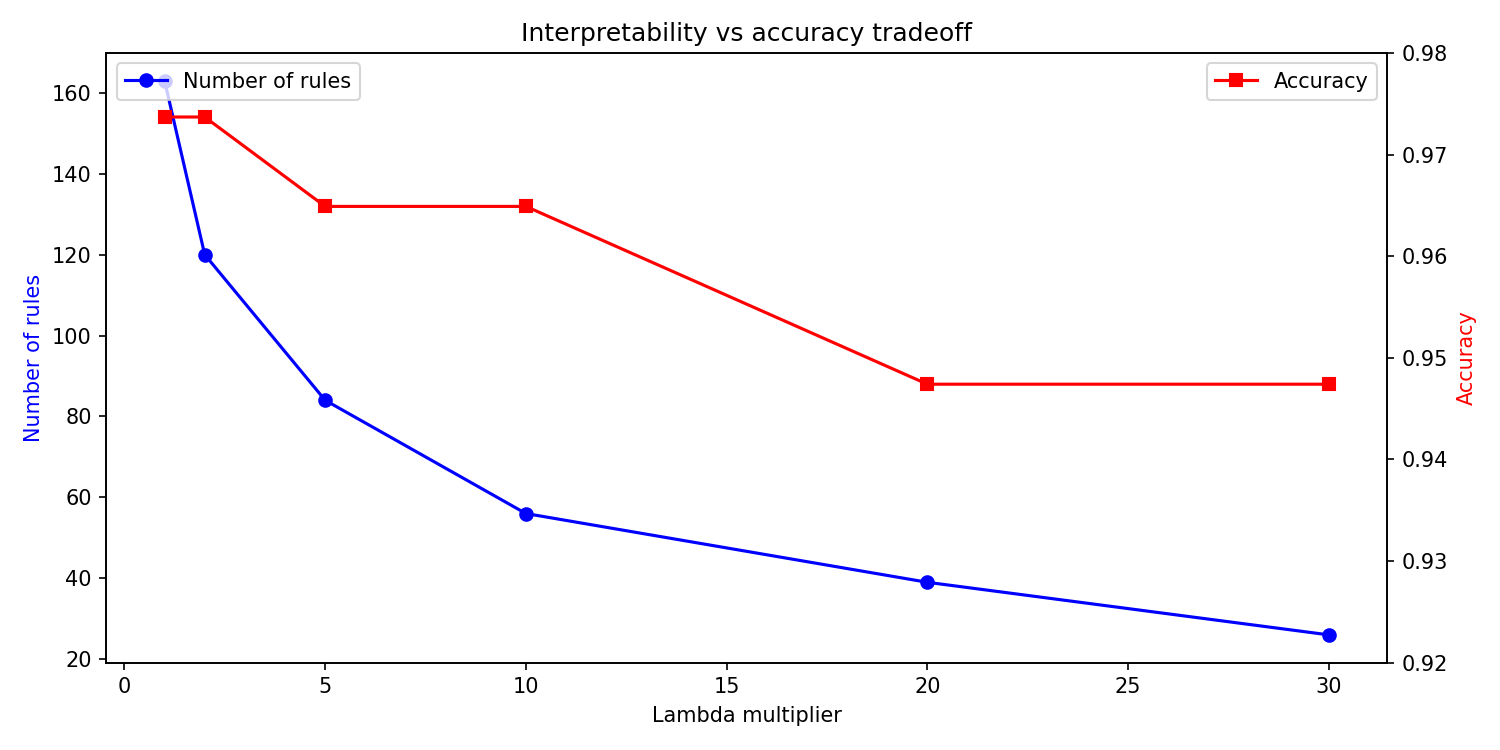
\includegraphics[width=\columnwidth]{tradeoff_curve.png}
\caption{Interpretability vs accuracy tradeoff on breast cancer (Lasso pipeline).}
\label{fig:bc-tradeoff}
\end{figure}

\begin{figure}[h]
\centering
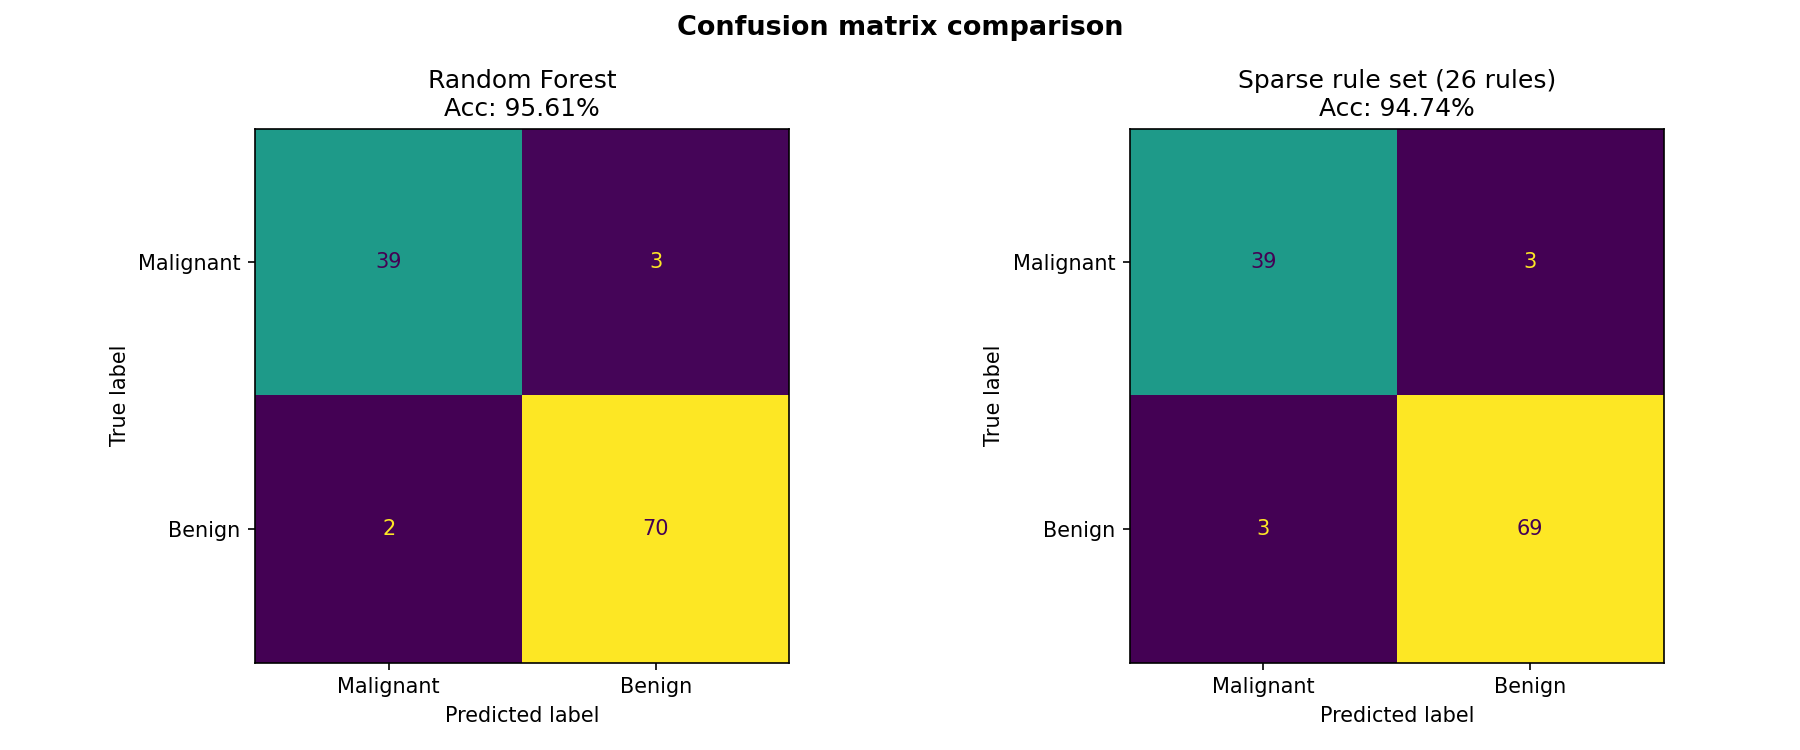
\includegraphics[width=\columnwidth]{confusion_matrices.png}
\caption{Confusion matrices: Random Forest (left) vs sparse rule set (right) on breast cancer.}
\label{fig:bc-cm}
\end{figure}

\subsection{Pima Indians Diabetes}

\begin{table}[h]
\centering
\small
\begin{tabular}{@{}lrrrr@{}}
\toprule
Method & \#rules & Acc & F1 & Recall$_+$ \\
\midrule
RF & --- & 0.7273 & 0.5625 & 0.5000 \\
Lasso & 20 & 0.7078 & 0.3836 & 0.2593 \\
RF (bal.) & --- & 0.7727 & 0.7009 & 0.7593 \\
Lasso (bal.) & 32 & 0.7532 & \textbf{0.7031} & \textbf{0.8333} \\
SIRUS & 12 & 0.7143 & 0.5417 & 0.4815 \\
SIRUS (bal.) & 10 & 0.6948 & 0.5841 & 0.6111 \\
\bottomrule
\end{tabular}
\caption{Pima diabetes results. Recall$_+$ denotes recall on the diabetic class.}
\label{tab:pima-results}
\end{table}

The Pima dataset is meaningfully harder. The Random Forest baseline reaches only 72.73\% accuracy, with diabetic recall of 0.50 reflecting the difficulty of separating diabetic from non-diabetic patients on this feature set.

The unbalanced Lasso pipeline retains 20 rules at $\lambda \times 10$, producing 70.78\% accuracy --- a 1.95\% drop from the baseline that would, looked at in isolation, suggest the pipeline transferred to this dataset cleanly. The aggregate metric is misleading. Per-class analysis shows that diabetic recall collapses from 0.50 (RF) to 0.26 (sparse rules) --- the rule set catches only one in four true diabetic patients. Inspection of the surviving rules reveals the cause: 15 of the 20 rules are non-diabetic-predicting and only 5 are diabetic-predicting. The Lasso, minimizing total mean squared error on a 65/35 training split, has learned that the loss-minimizing strategy is to predict the majority class far too often.

\subsubsection{Addressing the class-imbalance limitation}

We addressed the imbalance by setting \texttt{class\_weight=`balanced'} on the Random Forest and passing matching per-sample weights to \texttt{LassoCV}. The balanced sparse rule set contains 32 rules (11 diabetic-predicting, 21 non-diabetic-predicting), achieving 75.32\% accuracy, 0.7031 F1, and \textbf{0.83 diabetic recall} --- a 3.2$\times$ improvement on the metric that matters most in a clinical setting. The fix recovers most of what was lost without changing the dataset, the rule extraction algorithm, or the interpretability framework; only the loss-weighting changes. This finding is reported alongside the original numbers because the existence of the imbalance failure mode is itself a contribution: it argues that aggregate accuracy is an inadequate fidelity measure for any rule extraction method on imbalanced clinical data.

\subsubsection{SIRUS comparison}

SIRUS produces only 12 rules of 2 conditions each on Pima, reaching 71.43\% accuracy and 0.48 diabetic recall --- substantially better recall than unbalanced Lasso (0.26) without any explicit balancing. The shorter rules and fewer leaves naturally allocate more capacity to the minority class. Adding \texttt{class\_weight=`balanced'} pushes SIRUS recall to 0.61, with 10 rules. However, balanced Lasso still wins outright on F1 and recall, because longer rules can carve out more specifically-diabetic regions of the feature space.

\begin{figure}[h]
\centering
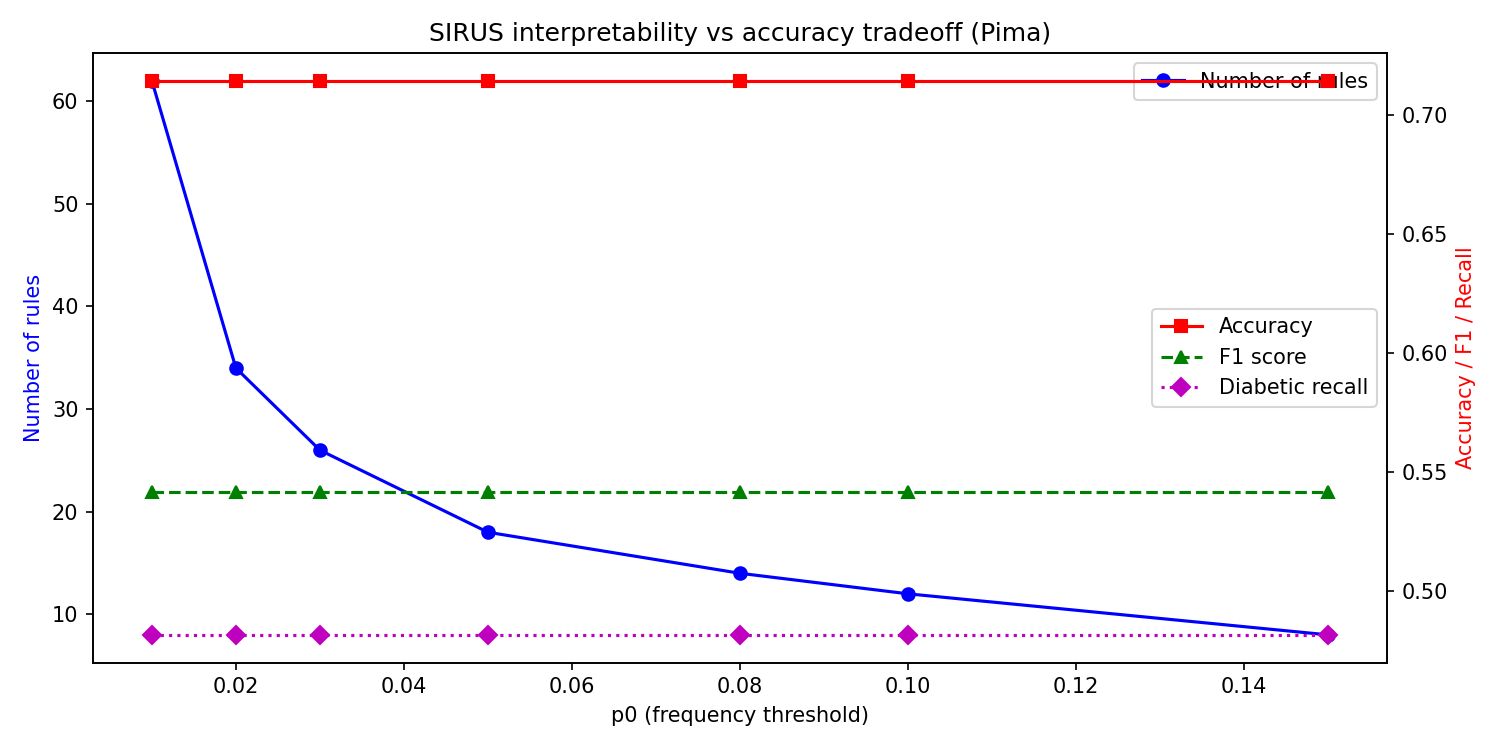
\includegraphics[width=\columnwidth]{sirus_pima_tradeoff.png}
\caption{SIRUS stability-threshold tradeoff on Pima. Increasing $p_0$ keeps only rules that appear more frequently across the forest.}
\label{fig:sirus-pima-tradeoff}
\end{figure}

\begin{figure}[h]
\centering
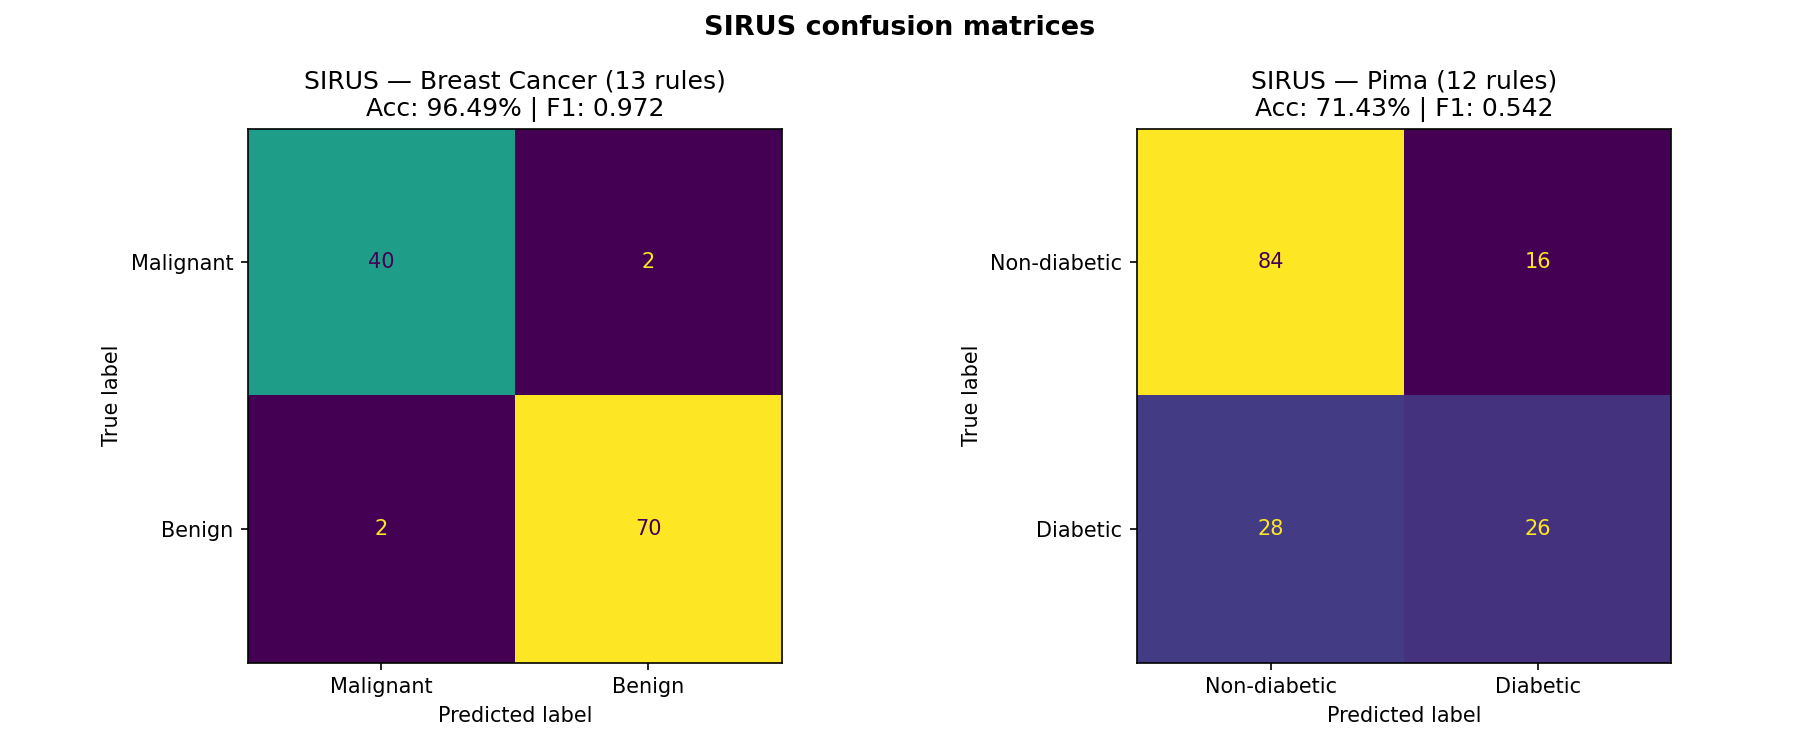
\includegraphics[width=\columnwidth]{sirus_confusion_matrices.png}
\caption{SIRUS confusion matrices comparing breast cancer and Pima diabetes performance.}
\label{fig:sirus-cm}
\end{figure}

\begin{figure}[h]
\centering
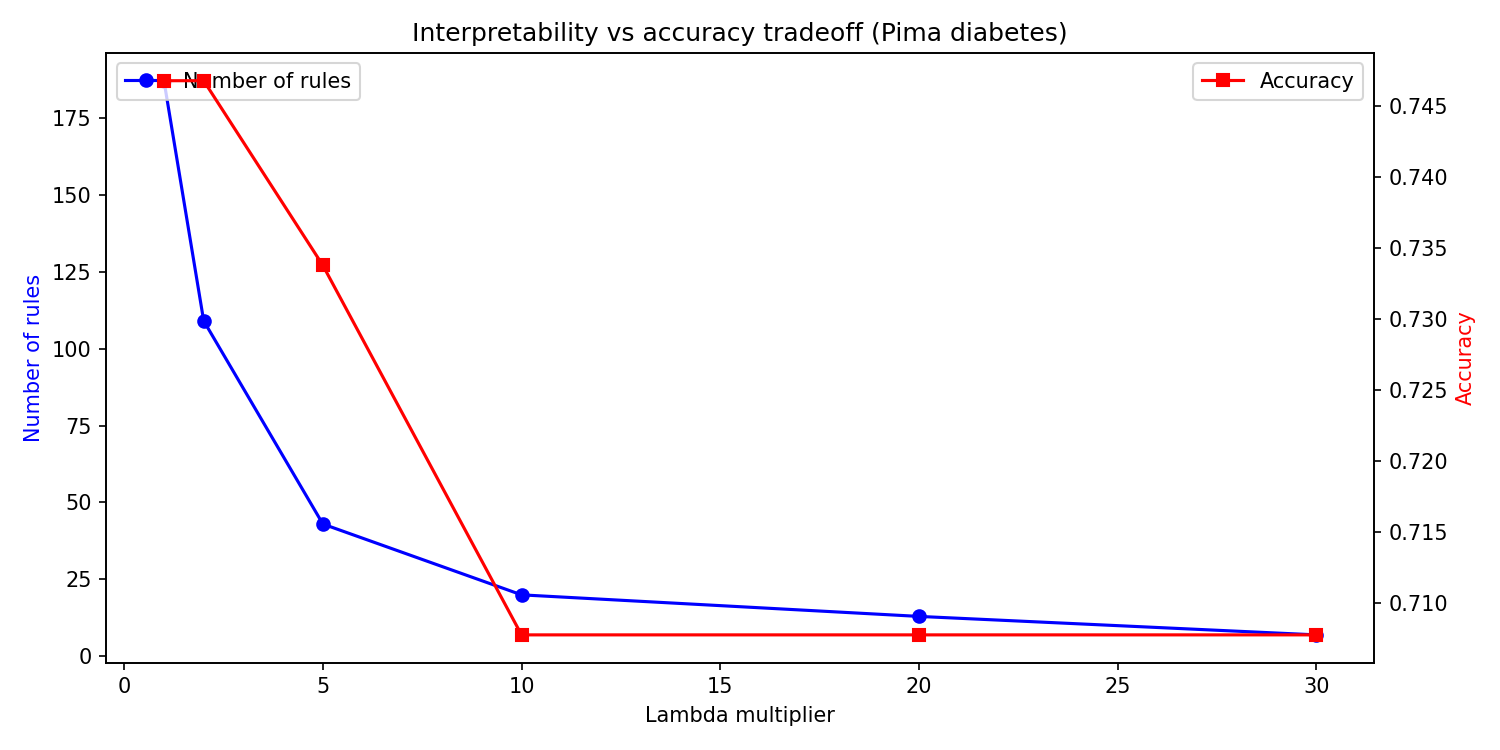
\includegraphics[width=\columnwidth]{pima_tradeoff_curve.png}
\caption{Interpretability vs accuracy tradeoff on Pima (Lasso pipeline).}
\label{fig:pima-tradeoff}
\end{figure}

\begin{figure}[h]
\centering
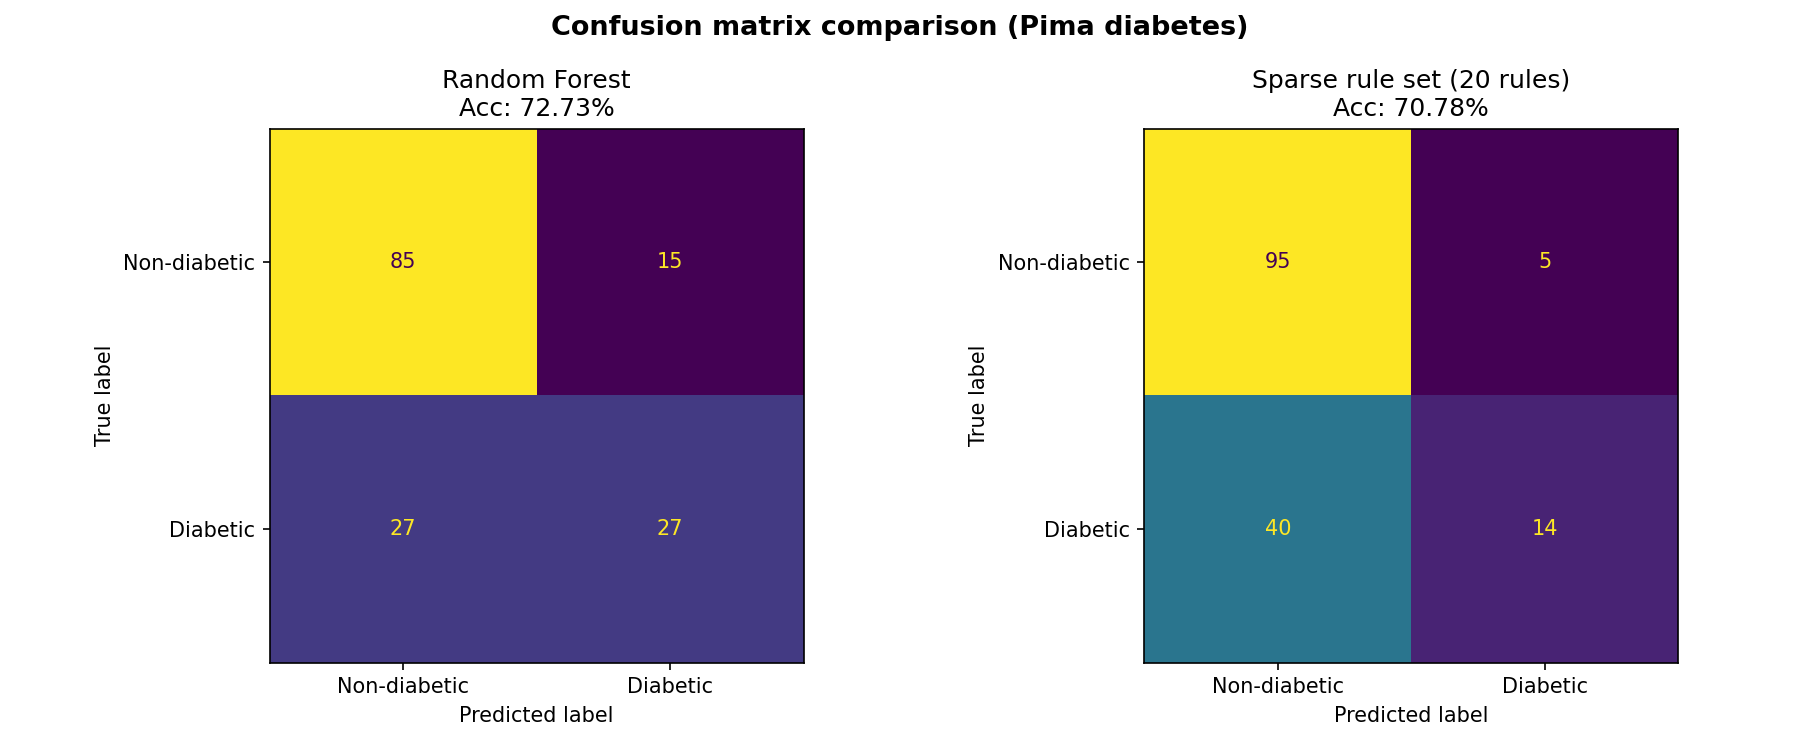
\includegraphics[width=\columnwidth]{pima_confusion_matrices.png}
\caption{Confusion matrices: Random Forest (left) vs unbalanced sparse rule set (right) on Pima.}
\label{fig:pima-cm}
\end{figure}

\subsection{Sanity Check: Do the Results Match Clinical Intuition?}

Beyond aggregate metrics, we examined whether the rules our pipeline selected align with what a clinician would expect, because a model that achieves the right accuracy for the wrong reasons is not useful in a clinical setting. On breast cancer, the most heavily-weighted rules condition on \texttt{mean concave points}, \texttt{worst perimeter}, \texttt{worst area}, and \texttt{radius error} --- features that capture the irregular, lobed boundary morphology characteristic of malignant tumors. These are the same descriptors a pathologist would highlight when explaining a diagnosis from biopsy imagery. On Pima, the strongest diabetic-predicting rule in the balanced model is approximately \textit{Glucose $>$ 154 AND BMI $>$ 23 AND Age $\leq$ 57 $\rightarrow$ Diabetic}, which matches the textbook risk profile for type-2 diabetes. The fact that both pipelines independently rediscovered clinically reasonable patterns --- without any clinical knowledge encoded in the algorithm --- is the strongest evidence that the rule extraction is capturing genuine structure rather than artifacts of how the trees happened to split. Where the results seem mathematically counterintuitive (the unbalanced Lasso ``losing'' on Pima despite a small accuracy drop) we have already traced the cause to the loss function under class imbalance rather than to a coding error or modelling failure.

\subsection{Structural feature alignment}

On both datasets, the features that appear in the sparse rule set match the Random Forest's own top Gini features almost completely: 8 of 8 on Pima (where the small feature space makes 100\% trivial) and a strong overlap on breast cancer (Figure~\ref{fig:bc-signal}). This validates that the extraction pipeline preserves the same structural signal the black box considered important, rather than picking up artifacts of the rule-counting procedure.

\begin{figure}[h]
\centering
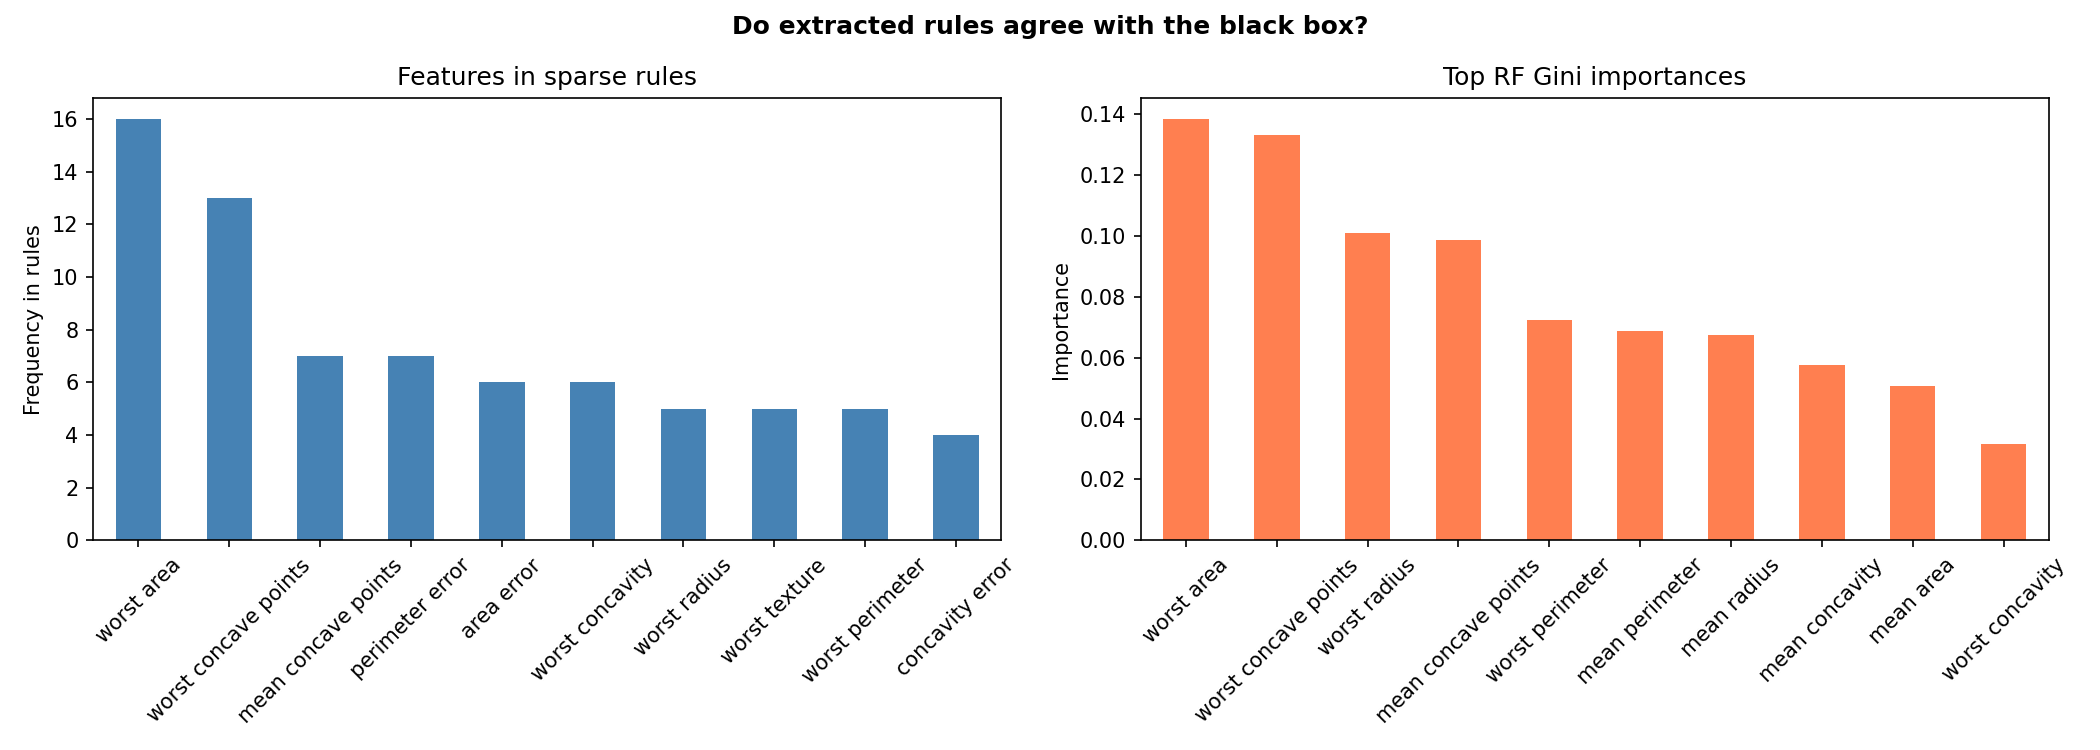
\includegraphics[width=\columnwidth]{signal_vs_noise.png}
\caption{Top-10 features in extracted rules (left) compared to top-10 Random Forest Gini importances (right) on breast cancer.}
\label{fig:bc-signal}
\end{figure}

\section{Discussion}

The two datasets tell complementary stories. On the clean, near-balanced breast cancer data, both rule extraction methods deliver compact, accurate, and clinically reasonable rule sets. SIRUS in fact \emph{outperforms} the Random Forest while using fewer rules with shorter conditions --- a striking result for an interpretable model and one the original SIRUS paper anticipates as the algorithm's intended sweet spot.

On the harder Pima diabetes data, the picture is nuanced. Vanilla Lasso, which appeared to transfer cleanly when judged by accuracy alone, in fact suffered a severe drop in minority-class recall that aggregate metrics hid. The reason is structural: $L_1$-regularized regression minimizes squared error over the training population, and on an imbalanced dataset the loss-minimizing rule set is one that predicts the majority class. We took this finding seriously rather than papering over it. The class-balancing fix is small in implementation effort (one parameter on the Random Forest, one sample-weight argument on Lasso) but recovers most of the lost recall, and demonstrates that the limitation is addressable without abandoning the rule-extraction framework.

The SIRUS comparison provides a useful counterpoint. Even without explicit balancing, SIRUS shows higher minority-class recall than vanilla Lasso, because shallower trees and fewer leaves force the algorithm to allocate prediction capacity more evenly across the input space. This suggests that the choice between Lasso and SIRUS is not a free choice; SIRUS is a more conservative, more stable algorithm whose biases happen to align well with imbalanced clinical data, while Lasso is a more flexible algorithm that can capture longer interactions but requires explicit balancing to do so safely.

A clear limitation of our current pipeline is that it inherits structural quirks from the underlying tree paths. Several extracted Lasso rules contain redundant inequalities on the same feature (e.g., one rule asks for both \texttt{Glucose > 154.5} and \texttt{Glucose > 165.5}; the first is implied by the second), an artifact of decision trees revisiting the same feature with tightening thresholds. A post-processing simplification step that collapses redundant inequalities would tighten the human-readability of the rule set without changing predictive behavior. Additionally, the Pima dataset contains zero-valued sentinels for several features that actually represent missing data; treating these as observed values during rule extraction silently contaminates the semantics of conditions like \texttt{Insulin <= 661}. Proper missing-data handling is a natural next step.

A second important caveat is statistical. With test sets of only 114 (breast cancer) and 154 (Pima) patients, the 95\% confidence intervals on accuracy and F1 are wide --- a difference of one or two percentage points between methods on a single 80/20 split should not be over-interpreted. A more rigorous follow-up would bootstrap the test predictions or repeat the train-test split across many random seeds and report mean $\pm$ standard deviation. We did not do this in the current analysis to keep the comparison numerically simple, and we flag it explicitly as a limitation on any claim that one method is strictly ``best'' on a given dataset. The headline qualitative findings --- the F1 collapse under class imbalance, the recovery under class-weighting, and the agreement between rule features and Gini importances --- are robust to this caveat because the effects are large; the smaller method-to-method gaps in Tables~\ref{tab:bc-results} and~\ref{tab:pima-results} are not.

\section{Conclusion}

We implemented and evaluated a complete post-hoc rule extraction pipeline that compresses a 100-tree Random Forest into a small set of human-readable IF-THEN rules. The pipeline supports two selection strategies --- $L_1$-regularized regression and frequency-based SIRUS --- and produces compact rule sets (12--32 rules) that retain the majority of the black-box's predictive accuracy on two clinical classification datasets.

The central finding is that interpretability has a measurable but bounded price, and that price varies with data structure. On clean, balanced data, the price is essentially zero. On imbalanced clinical data, the naive pipeline appears to transfer cleanly when judged by accuracy alone but in fact loses most of its minority-class recall; addressing this requires explicit class-weighted training, after which the framework recovers gracefully. Both rule-selection methods produce rule sets that align strongly with the Random Forest's own feature importances, validating that the extraction process captures genuine signal rather than noise.

Future work includes implementing rule simplification to remove redundant conditions, handling missing-value sentinels in the Pima dataset, and extending the pipeline to multi-class clinical settings where conflict resolution becomes more delicate.

\begin{thebibliography}{7}

\bibitem[Breiman(2001)]{breiman2001randomforests}
Leo Breiman. 2001.
\newblock Random forests.
\newblock \textit{Machine Learning}, 45(1):5--32.

\bibitem[B\'enard et~al.(2021)]{benard2021sirus}
Cl\'ement B\'enard, G\'erard Biau, S\'ebastien da~Veiga, and Erwan Scornet. 2021.
\newblock SIRUS: Stable and interpretable rule set for classification.
\newblock \textit{Electronic Journal of Statistics}, 15(1):427--505. (arXiv:1908.06852).

\bibitem[Friedman and Popescu(2008)]{friedman2008rule}
Jerome H. Friedman and Bogdan E. Popescu. 2008.
\newblock Predictive learning via rule ensembles.
\newblock \textit{The Annals of Applied Statistics}, 2(3):916--954.

\bibitem[Pedregosa et~al.(2011)]{pedregosa2011sklearn}
Fabian Pedregosa, Ga\"el Varoquaux, Alexandre Gramfort, Vincent Michel, Bertrand Thirion, Olivier Grisel, et~al. 2011.
\newblock Scikit-learn: Machine learning in Python.
\newblock \textit{Journal of Machine Learning Research}, 12:2825--2830.

\bibitem[Smith et~al.(1988)]{smith1988pima}
Jack~W. Smith, J.~E. Everhart, W.~C. Dickson, W.~C. Knowler, and R.~S. Johannes. 1988.
\newblock Using the ADAP learning algorithm to forecast the onset of diabetes mellitus.
\newblock In \textit{Proceedings of the Symposium on Computer Applications in Medical Care}, pages 261--265.

\bibitem[Tibshirani(1996)]{tibshirani1996lasso}
Robert Tibshirani. 1996.
\newblock Regression shrinkage and selection via the lasso.
\newblock \textit{Journal of the Royal Statistical Society: Series B}, 58(1):267--288.

\bibitem[Wolberg et~al.(1995)]{wolberg1995breastcancer}
William~H. Wolberg, W.~Nick Street, and Olvi~L. Mangasarian. 1995.
\newblock Breast Cancer Wisconsin (Diagnostic) Data Set.
\newblock UCI Machine Learning Repository.

\end{thebibliography}

\end{document}
